\chapter{Implémentation en C++ et problèmes rencontrés}

Ce chapitre a pour but d'aider les prochains qui souhaiteraient coder en C++ pour qu'ils ne se heurtent pas aux même écueils que nous, et qu'ils puissent passer plus de temps sur la conception du projet plutôt que sur le debug et la recherche d'outils efficaces.

\section{Outils utilisés}

\subsection{IDE}

Il est important que chaque membre développe dans un IDE qui lui soit familier, et qui offre un minimum d'ergonomie et d'efficacité. Dans le projet, les IDE utilisés ont été :
\begin{itemize}
    \item Xcode, pour développer sous Mac (et utilisation de Clang au lieu de LLVM pour les parallélisations OpenMP \cite{menshov_xcode_2017} ). 
    \item QtCreator, disponible sous Linux et Windows (bien qu'il soit un peu plus pénible à installer sous Windows).
    \item Vim, déconseillé à ceux qui ne maîtrisent pas l'outil, mais qui peut se révéler très puissant avec les bons plugins.
\end{itemize}

Chaque IDE venant avec ses propres fichiers de configuration, nous conseillons de nommer ceux-ci du nom de leur utilisateur (typiquement john\_doe.pro.user) ou de les ajouter au .gitignore afin d'éviter les conflits.

\subsection{Conseils à de futurs groupes}
\paragraph{Language de programmation}
Outre le fait que nous déconseillons vivement aux futurs membres de ce projet long d'utiliser un langage qui ne soit pas maîtrisé par au moins la moitié de l'équipe, nous avons proposé au corps encadrant, après un passage obligatoire par un langage de programmation afin de comprendre la structure des réseaux neuronaux, de faire passer à des framework de \textit{machine learning}, tels que PyTorch ou Keras+TensorFlow, afin de réduire les risques de problèmes de codes survenant dans l'implémentation des réseaux neuronaux plus complexes.
\paragraph{Bonnes pratiques}
Nous conseillons aux membres du groupe d'adopter dès le début de bonnes pratiques, qui ont pu être source de conflit les années précédentes ou simplement afin d'éviter de produire du code pouvant larguer d'autres membres du groupe. Quelques unes sont listées ci-dessous :
\begin{itemize}
\item Adopter une convention de syntaxe de programmation par défaut.
\item Mettre en place une documentation générée par Doxygen (on conseille le module plantUML pour la génération automatique de parties du diagramme UML). 
\item Faire usage des merge/pull requests validé par autrui
\end{itemize}

\subsection{Affichage des résultats}
Les images et courbes étaient initialement manuellement obtenues depuis des modèles de fichiers Excel.
Afin de ne pas avoir à coder une seule ligne du language hérétique qu'est Python et son module GnuPlot, nous avons écrit un simple script bash (disponible sur le dépôt github) exploitant GnuPlot pour l'affichage des résultats. 
\begin{figure}[!h]
\begin{center}
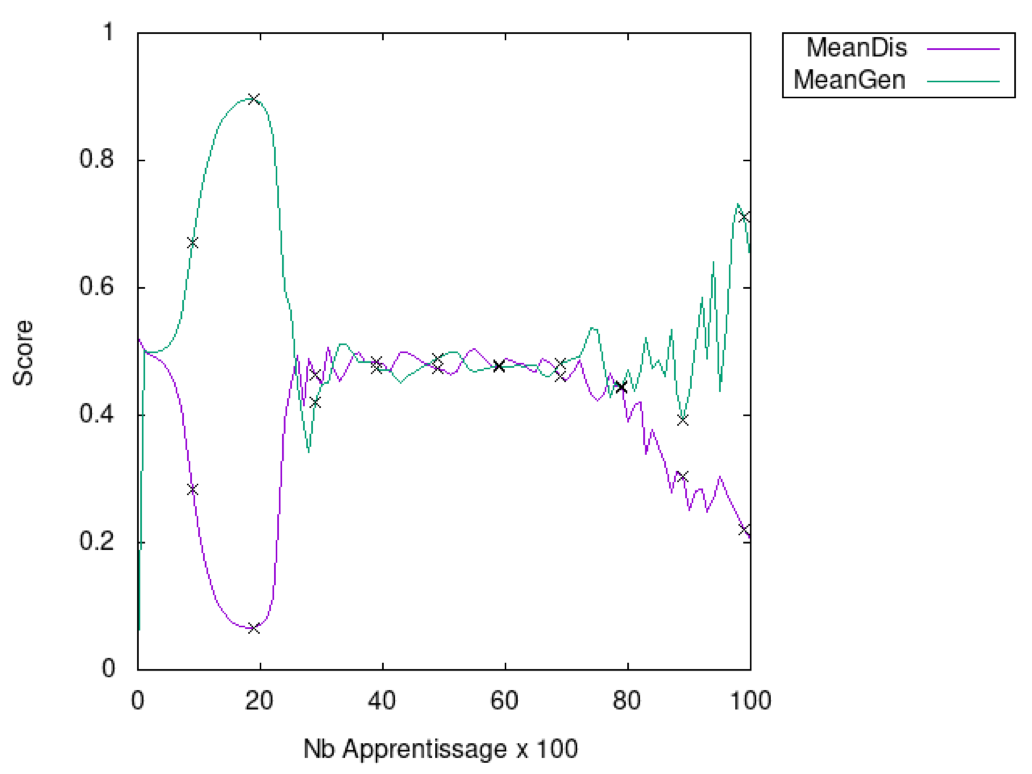
\includegraphics[width=0.7\textwidth]{images/18_02_22-GnuPlot.png}
\caption{Un exemple d'une exportation GnuPlot}
\label{fig:type-appr-GAN}
\end{center}
\end{figure} 
\subsection{Rapport}
Le rapport est fait sous LaTeX, avec des éditeurs et compilateurs en local ou via Overleaf (et son module git) ou Sharelatex (et son module Gitlab). La bibliographie BibTex est générée à partir de l'export de la base de donnée de documents Zotero. La compilation vers PDF en CI n'a pas été faite car Travis-CI ne le prend pas en charge facilement (nécessité de réinstaller latex sur les images docker à chaque compilation, ce qui est beaucoup trop lent). La compilation aurait été faisable, en utilisant une image gitlab-ci latex, si le projet avait été hosté sur Gitlab.com.

\section{C++ et Problèmes rencontrés}
\subsection{C++11}
Un des groupes précédents \cite{amosse_pinapl_2017} ayant codé en C++ ont perdu une bonne partie de leur année à débugger des fuites de mémoire, dû à la gestion de pointeurs sous C++98. Nous sommes donc parti sur C++11 afin de faire un usage extensif des \textit{smart pointers}
N.B. Ce même groupe a perdu une autre bonne partie de l'année à vouloir recoder la multiplication marticielle et à la débugger. C'est la raison de la section ci-dessous 


\subsection{Eigen}
Les réseaux de neurones de type perceptron reposent largement sur les produits matriciels. Afin d'effectuer ces calculs le plus efficacement possible, notre code utilise le framework C++ Eigen. Ce framework permet de manipuler l'algèbre linéaire et les matrices de manière la plus optimale possible. De plus, Eigen utilise OpenMP ce qui permet de paralléliser les calculs sur l'ensemble des cœurs. 

De ce que nous avons pu voir, il n'existe aucune alternative à Eigen qui offre autant de possibilités et d'optimisation. Cependant Eigen n'est pas facile à manipuler au premier abord. Sa construction est entièrement à base de template et est organisée de façon à pouvoir effectuer le plus de calculs possible en compile-time, ce qui rend les types des objets et les messages d'erreur difficilement déchiffrables. Débugger un problème lié à Eigen nécessite un bon débogueur et de la patience. 

\paragraph{Particularités}
La classe Eigen::MatrixXf ne sait pas faire du coefficient par coefficient, il faut passer par la classe Eigen::ArrayXf par une conversion
soit : (matrice1.array() * matrice2.array()).matrix()…
\paragraph{Parallélisation des calculs}
De plus, la méthode de parallélisation d'Eigen reste assez obscure. Le framework semble paralléliser les calculs en colonnes, c'est à dire qu'il calcule simultanément les colonnes de la matrices résultante d'un calcul. Autrement dit, si le résultat est une ligne, le calcul sera parallélisé, mais si c'est une colonne il ne tournera que dans un seul thread. Ceci implique de n'utiliser que des matrices lignes dans le code, bien que tous les calculs menés théoriquement soient faits avec des colonnes. Attention donc à transposer correctement.
\paragraph{Convolution}\label{implementation-C++-convolution}
Contrairement à Numpy, Eigen ne traite pas la convolution, il est nécessaire de la coder à la main. Cela nous a ralenti dans l'avancement du projet et dans l'obtention de résultats, notamment pour CIFAR qui nécessite des étapes de convolution.